% !TEX root = Master.tex

A crucial part of this study is the cluster analysis of the forest compartments. Therefore, we perform simple k-means clustering on the compartments to resolve a key issue: The single compartments themselves do not have enough
observations to perform any kind of distribution fitting via Maximum Likelihood Estimation. Clustering relatively similar compartments could resolve
this issue by creating k clusters, whereby each cluster then has enough observations to perform distribution fitting.\\

The following auxiliary variables are assigned to each of the compartments to calculate distances. The thought process of those variables to describe the systematic bias is further outlined in Table \ref{tab:auxiliary_variables}.

\begin{table}[H]
\setlength\arrayrulewidth{1pt}
\centering
\begin{adjustbox}{max width=\textwidth}
\begin{tabular}{|c|c|}
\hline
\rowcolor{Gray}
\textbf{Variable}                                                                              & \textbf{Potential to explain Bias}                                                                                                                                   \\ \hline
\begin{tabular}[c]{@{}c@{}}Forest Cover Ratio\\ Area / \# of Detected Trees\end{tabular}       & \multirow{2}{*}{\begin{tabular}[c]{@{}c@{}}A densely forested region will have more dominant\\ subdominant structures.\end{tabular}}                                 \\ \cline{1-1}
\begin{tabular}[c]{@{}c@{}}Tree crown coverage\\ Area surface  - Total Crown Area\end{tabular} &                                                                                                                                                                      \\ \hline
Variation of crown area                                                                        & \multirow{2}{*}{\begin{tabular}[c]{@{}c@{}}Large variation in the Tree Crowns and overall large crowns\\ will have more dominant subdominant structure\end{tabular}} \\ \cline{1-1}
0.75 quantile of crown area                                                                    &                                                                                                                                                                      \\ \hline
Variation of height                                                                            & \begin{tabular}[c]{@{}c@{}}If the cultivation time is similar, the trees should be of same\\ height, resulting in less covering\end{tabular}                         \\ \hline
\end{tabular}
\end{adjustbox}

\caption{Auxiliary variables for k-mean clustering}
\label{tab:auxiliary_variables}
\end{table}

All variable combinations were tested by a time-consuming trial-and-error procedure. Meaning that for each
generated cluster output, a Principle Component Analysis is performed (if > 2 variables), visualizing the goodness
of separation from each group (Figure \ref{fig:Clusterplot}). Subsequently 3-D plots from the LiDAR dataset for
several compartments of each cluster are created. Clustering is considered successful, once the groups can be well
explained by the 3-D images and the separation of the clusters is reasonable.\\
This is presented with the final model used in this study.\\

\begin{figure}[H]
\centering
  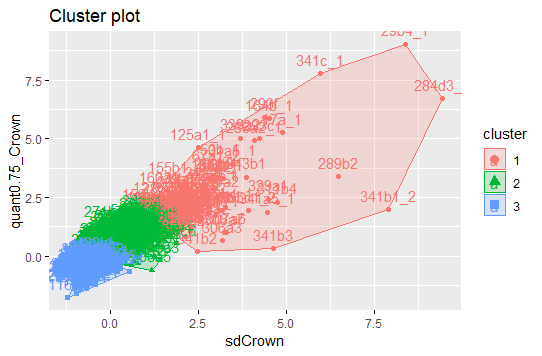
\includegraphics[scale = 0.85]{clusterplot.png}
  \caption{Scatterplot of the sections with the grouping based on k-means clustering}
  \label{fig:Clusterplot}
\end{figure}

The chosen final auxiliary variables are the 0.75 quantile of the crown area and the variation of the crown area.
Figure \ref{fig:Clusterplot} shows high correlation. This is additionally depicted in Figure \ref{fig:Boxplots Cluster}. The desired property of a clear separation of the clusters is not fully given. We render this as a
minor problem. The three cluster are large enough so that enough samples from inventory data are in each
cluster. Cluster 1 336, cluster 2 4180, cluster 3 5471.\\

\begin{figure}[H]
\centering
  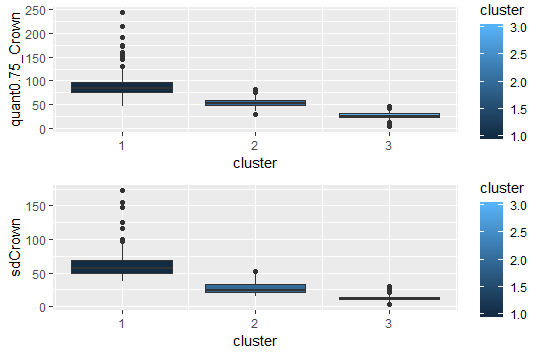
\includegraphics[scale = 0.85]{boxplots_cluster.png}
  \caption{Boxplots for the used variables - clusters}
  \label{fig:Boxplots Cluster}
\end{figure}


The 3-D plots of some compartments for each cluster offer insights into the goodness of the clustering. Sections in
cluster 1 appear to be very dense areas as the forests soil is barely visible. Interestingly, the tree height appears
to be rather equal, resulting in homogeneous patches. This is well depicted by compartment 261a2 (Figure \ref{fig:LiDAR Cluster 1}). The
compartment in cluster 2 are sparser wooded (Figure \ref{fig:LiDAR Cluster 2}). Blue patches (forest soil) are visible in every compartment. This is even
stronger pronounced in the compartments of cluster 3 (Figure \ref{fig:LiDAR Cluster 3}).


\begin{figure}[H]
  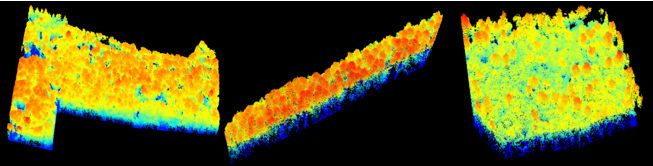
\includegraphics[width=\textwidth]{cluster1_lidar.png}
  \caption{Cluster 1 section ID's from left to right: 155a1, 311b1, 261a2}
  \label{fig:LiDAR Cluster 1}
\end{figure}

\begin{figure}[H]
  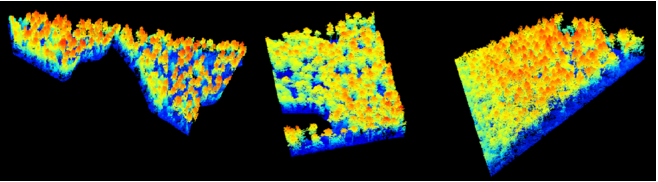
\includegraphics[width=\textwidth]{cluster2_lidar.png}
  \caption{Cluster 2 section ID's from left to right: 37a2, 71b5, 309a2}
  \label{fig:LiDAR Cluster 2}
\end{figure}

\begin{figure}[H]
  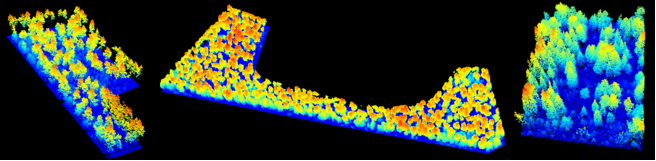
\includegraphics[width=\textwidth]{cluster3_lidar.png}
  \caption{ Cluster 3 section IDs from left to right: 314a2, 207a2, 36c1}
  \label{fig:LiDAR Cluster 3}
\end{figure}

Using the variable tree crown to describe the clusters is difficult. No actual difference in the variation and quantile
of the crown area between the clusters can be observed visually. Anyhow, dense and sparse
forested region are well separated.\\

It might be explained as following. Dense compartments show regions of equally height trees. The tree detection
algorithm is unable to detect all trees, as tree crowns of several trees are detected as one (see Section \ref{Challenges}). This
leads to unnatural high variation in the crown area. The quantile of the crown area further captures the extent of
this effect.

